\textbf{LeVeque 2.4} 

a) Modify the m-file \texttt{bvp2.m} so that it implements a Dirichlet boundary condition at $x = a$ and a Neumann
   condition at $x = b$ and test the modified program.

\begin{solution}\ \\\\
   For each step size $h$, our errors (and corresponding least squares fit) are as follows:\footnote{
      Differences between \texttt{problem\_4a.m} and source \texttt{bvp2.m} file can be found in
      \texttt{problem\_4a.diff}. 
   }\\
     
   \begin{lstlisting}[language=bash, basicstyle=\tiny]
      h        error       ratio       observed order
   0.30000   1.74886e+00       NaN             NaN
   0.15000   4.80811e-01   3.63732         1.86288
   0.07500   1.26086e-01   3.81336         1.93106
   0.03750   3.22858e-02   3.90531         1.96544

Least squares fit gives E(h) = 18.0049 * h^1.92092
   \end{lstlisting}

   \begin{figure*}[h]
        \centering
        \begin{subfigure}[b]{0.475\textwidth}
            \centering
            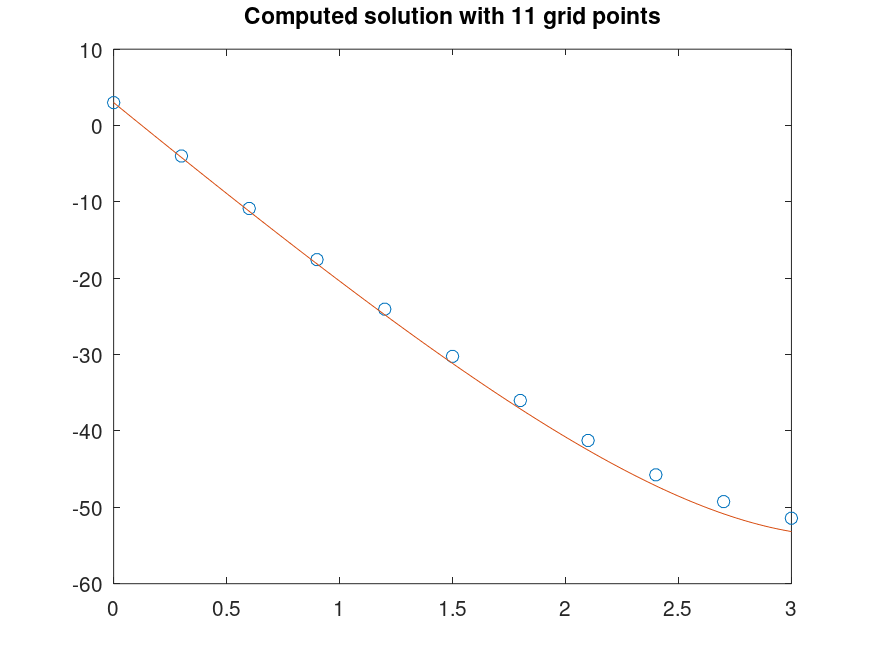
\includegraphics[width=\textwidth]{problem4a_11_grid_points.png}
            \caption[]%
            {{\small $h = 0.30$}}    
            \label{fig:problem4a_11pt}
        \end{subfigure}
        \hfill
        \begin{subfigure}[b]{0.475\textwidth}
            \centering
            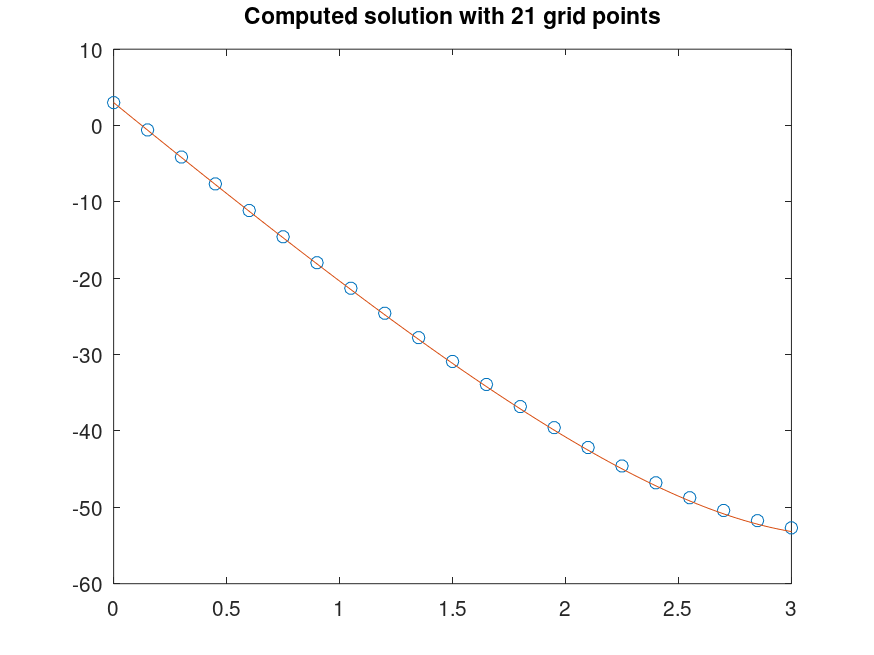
\includegraphics[width=\textwidth]{problem4a_21_grid_points.png}
            \caption[]%
            {{\small $h = 0.15$}}    
            \label{fig:problem4a_21pt}
        \end{subfigure}
        \vskip\baselineskip
        \begin{subfigure}[b]{0.475\textwidth}
            \centering
            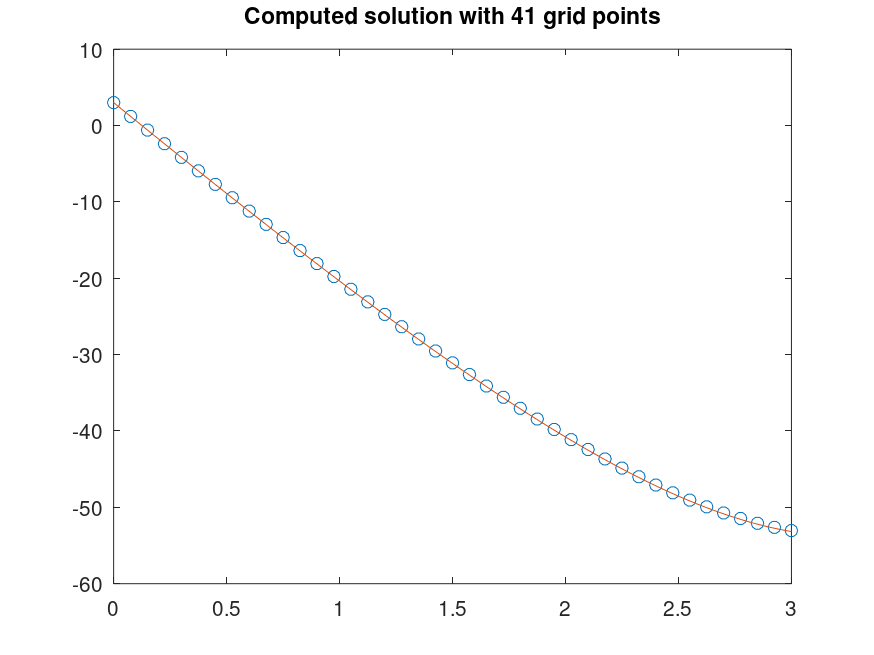
\includegraphics[width=\textwidth]{problem4a_41_grid_points.png}
            \caption[]%
            {{\small $h = 0.075$}}    
            \label{fig:problem4a_41pt}
        \end{subfigure}
        \hfill
        \begin{subfigure}[b]{0.475\textwidth}
            \centering
            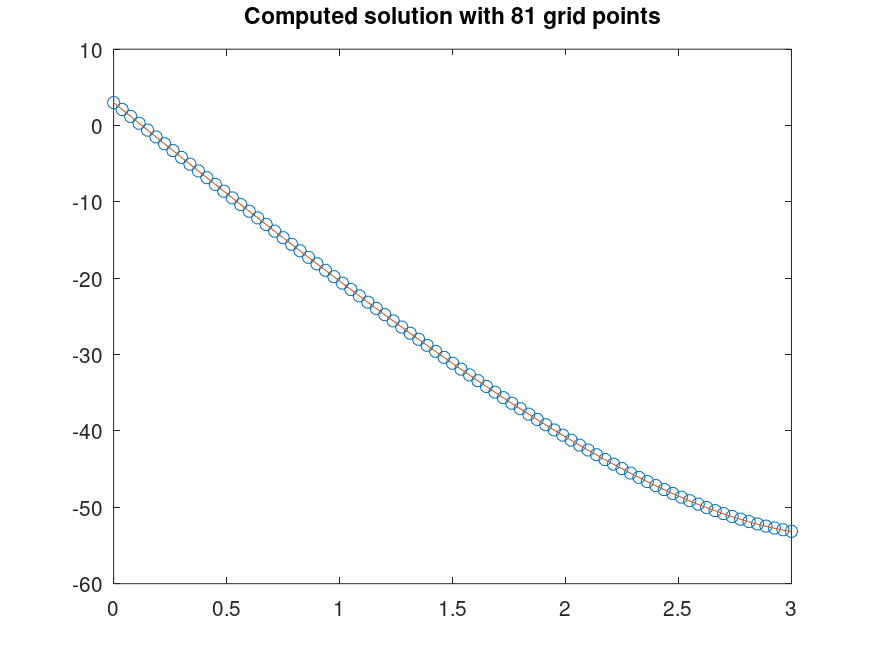
\includegraphics[width=\textwidth]{problem4a_81_grid_points.png}
            \caption[]%
            {{\small $h = 0.0375$}}    
            \label{fig:problem4a_81pt}
        \end{subfigure}
        \caption[ The average and standard deviation of critical parameters ]
        {\small Computed second-order solution to $u''(x) = e^x$ with Dirichlet and Neumann BCs} 
        \label{fig:bvp2}
   \end{figure*}
\end{solution}

\pagebreak
b) Make the same modification to the m-file \texttt{bvp4.m}, which implements a fourth order accurate method. Again test
   the modified program.

\begin{solution}\ \\\\
   For each step size $h$, our errors (and corresponding least squares fit) are as follows:\footnote{
      Differences between \texttt{problem\_4b.m} and source \texttt{bvp4.m} file can be found in
      \texttt{problem\_4b.diff}. 
   }\\
     
   \begin{lstlisting}[language=bash, basicstyle=\tiny]
      h        error       ratio       observed order
   0.30000   7.22610e-02       NaN             NaN
   0.15000   5.21206e-03  13.86421         3.79329
   0.07500   3.47061e-04  15.01768         3.90859
   0.03750   2.23260e-05  15.54516         3.95839
 
 
Least squares fit gives E(h) = 8.04934 * h^3.88894
   \end{lstlisting}

   \begin{figure*}[h]
        \centering
        \begin{subfigure}[b]{0.475\textwidth}
            \centering
            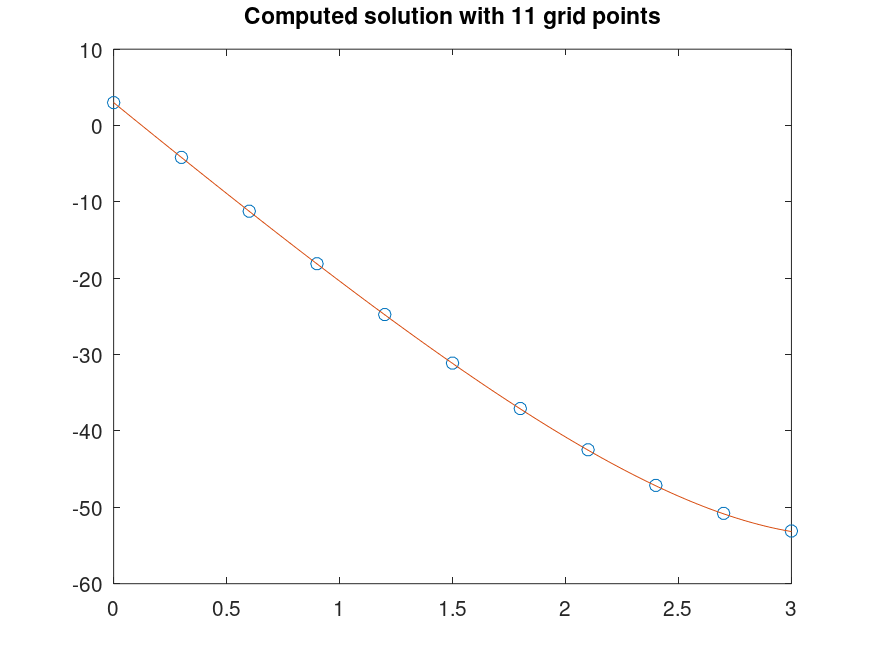
\includegraphics[width=\textwidth]{problem4b_11_grid_points.png}
            \caption[]%
            {{\small $h = 0.30$}}    
            \label{fig:problem4b_11pt}
        \end{subfigure}
        \hfill
        \begin{subfigure}[b]{0.475\textwidth}
            \centering
            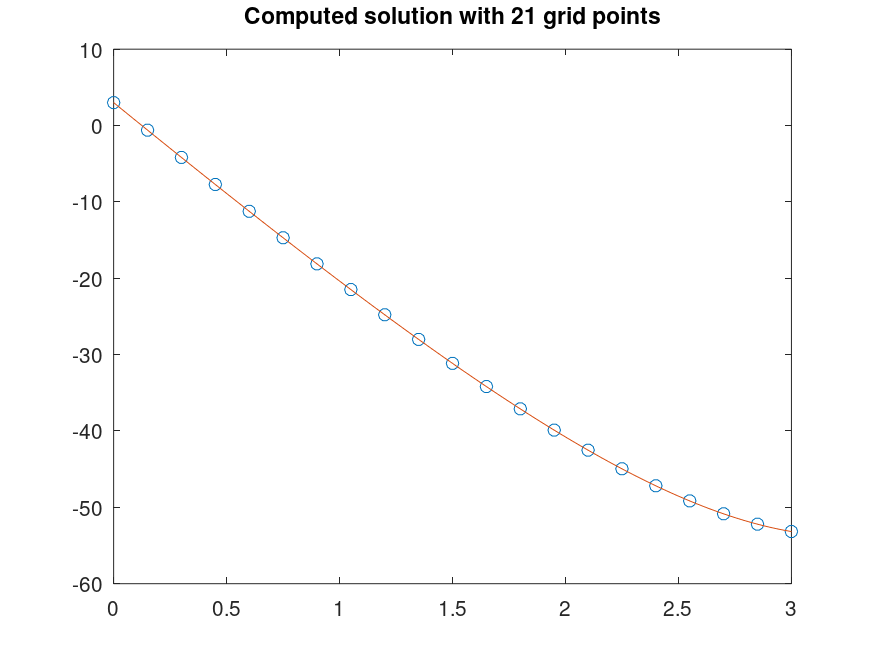
\includegraphics[width=\textwidth]{problem4b_21_grid_points.png}
            \caption[]%
            {{\small $h = 0.15$}}    
            \label{fig:problem4b_21pt}
        \end{subfigure}
        \vskip\baselineskip
        \begin{subfigure}[b]{0.475\textwidth}
            \centering
            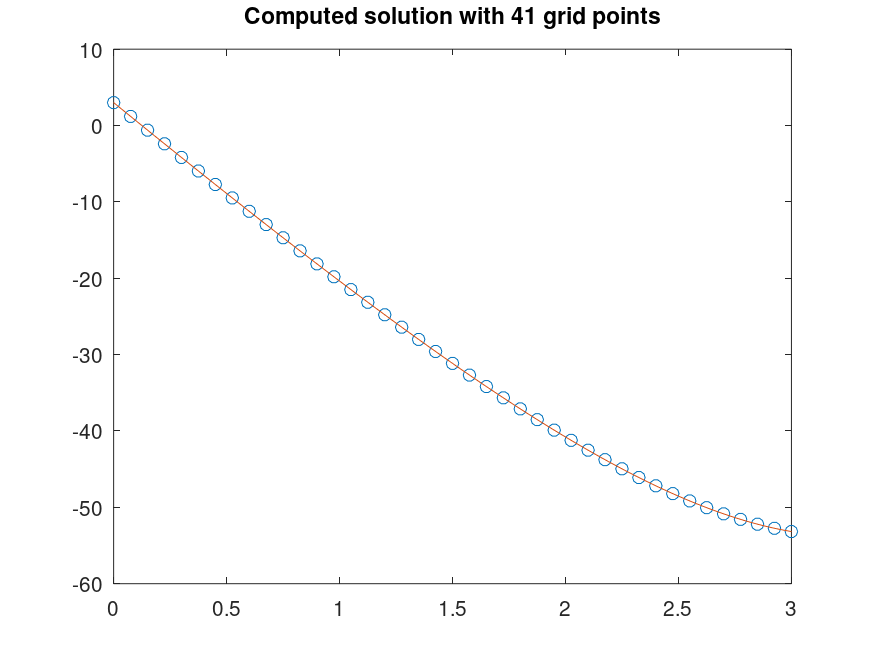
\includegraphics[width=\textwidth]{problem4b_41_grid_points.png}
            \caption[]%
            {{\small $h = 0.075$}}    
            \label{fig:problem4b_41pt}
        \end{subfigure}
        \hfill
        \begin{subfigure}[b]{0.475\textwidth}
            \centering
            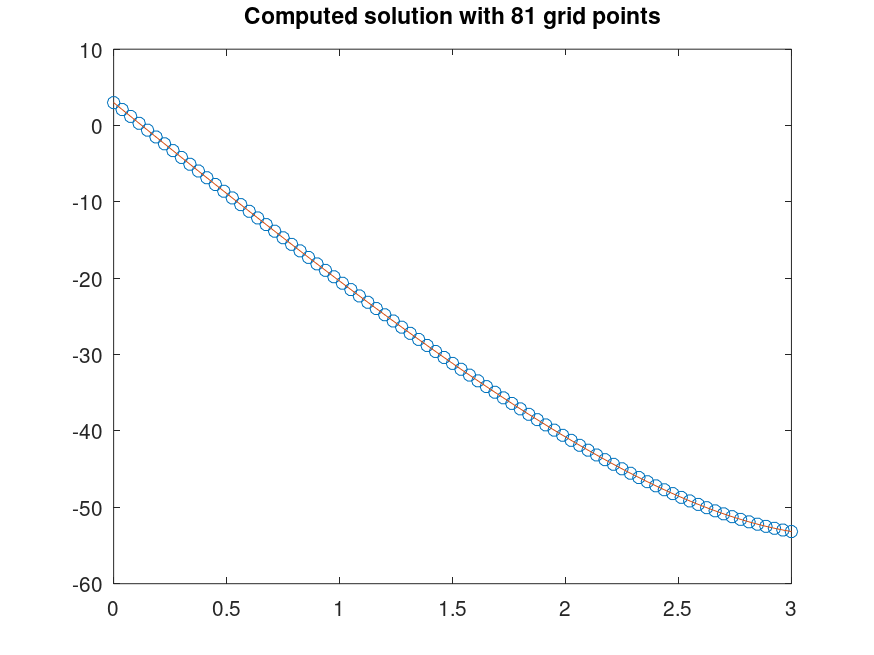
\includegraphics[width=\textwidth]{problem4b_81_grid_points.png}
            \caption[]%
            {{\small $h = 0.0375$}}    
            \label{fig:problem4b_81pt}
        \end{subfigure}
        \caption[ The average and standard deviation of critical parameters ]
        {\small Computed fourth-order solution to $u''(x) = e^x$ with Dirichlet and Neumann BCs} 
        \label{fig:bvp4}
   \end{figure*}
\end{solution}